\documentclass[nojss]{jss}
\usepackage{lifecon}
\usepackage{graphicx}
\usepackage{amsmath}
\usepackage{hyperref}
\usepackage[utf8]{inputenc}
% \usepackage{draftwatermark}
% \SetWatermarkText{Draft}
% \SetWatermarkScale{1.5}

%\usepackage{myVignette}
%\VignetteIndexEntry{Mortality projection using lifecontingencies package}
%%\VignetteDepends{lifecontingencies}
%%\VignetteKeywords{mortality projection, lifecontingencies, R}
%%\VignettePackage{lifecontingencies}
% need no \usepackage{Sweave.sty}
%\SweaveOpts{prefix.string=Figures/fig}

\author{Giorgio Alfredo Spedicato, ACAS \And 
        Gian Paolo Clemente, Unicatt}


\title{Mortality projection with \pkg{demography} and \pkg{lifecontingencies}
packages}

\Plainauthor{Giorgio Alfredo Spedicato, Gian Paolo Clemente}
\Plaintitle{Mortality projection with demography and lifecontingencies packages}
\Shorttitle{Mortality projection in \proglang{R}}
\Keywords{mortality projection, lifecontingencies, \proglang{R}}
\Plainkeywords{mortality projection, lifecontingencies, R}



\Abstract{
This paper applies mortality projection techniques
(Lee Carter) to the evaluation of retirement costs. The main purpose of the
paper is to show how R can be successfully used to perform life
expectancy projections with practical actuarial applications for annuity
insurances and social security issues. \pkg{demography} and
\pkg{lifecontingencies} packages will be used. The analysis performed within
this paper are mechanical and intended for didactic purposes.}

\Keywords{annuities, Lee-Carter, mortality projection, \pkg{lifecontingencies}, \pkg{demography}}
\Plainkeywords{annuities, Lee-Carter, mortality projection, lifecontingencies, demography} %% without formatting



\Address{
  Giorgio Alfredo Spedicato\\
  Ph.D ACAS C.STAT\\
  Via Firenze 11
  20037 Italy\\
  E-mail: \email{spedygiorgio@gmail.com}\\
  URL: \url{https://github.com/spedygiorgio/lifecontingencies}
}

\Address{Gian Paolo Clemente\\
  Catholic University of Milan\\
  Department of Mathematics, Finance and Econometrics
\email{gianpaolo.clemente@unicatt.it}
}

\begin{document}





\section{Introduction}
Mortality data shows that mortality is falling at all ages with a different behaviour according to different ages and country.
Mortality across any ages is indeed showing continuous reduction across the world. \\ 
Prospects of longer life have led to concern over their implications for public spending on old-age support. Forecasting mortality appears indeed a key issue in different field of insurance and financial markets as pricing annuity, evaluating mortality-linked securities and quantifying longevity risk. Lee-Carter proposed in 1992 a model widely used in order to forecast mortality rates.\\
The Lee Cartel forecasts could be used to project a life table for each specific cohort (year) of birth on which pension annuities projection could be fit.\\

Our exercise will be based on Italian data downloaded from the Human Mortality Databases (HMD) via \textbf{demography} (\cite{demographyR}) package dedicated function. We will use \textbf{demography} and \textbf{forecast} package in order to fit Lee - Carter model and perform 100 - years in advance extrapolations.\\
Finally, \textbf{lifecontingencies} (\cite{spedlifecon}) package will be used to project the cost of a pension annuity, $\ddot{a}_{x}^{(m)}$ for the cohorts of 1920, 1930, \ldots,
2000. \\ 
Applications have been provided by using three different data-sets regarding respectively male, female and total population.
The use of several data-sets is usually motivated by both the need of a separate evaluation between males and females and of an analysis of models' performance when switching data. However, the change from female to male and a variation in the length of period of observation do not influence the quality of fit as much as the restriction of age range.\\

Following demographic and economic assumptions will be hold:
\begin{itemize}
  \item $x$, the retirement age will be set equal to 65 regardless the cohort.
  \item $m$, the number of fractional payments per year, will be equal to 12.
  \item $\ddot{a}_{x}^{(m)}$ to be the actuarial present value of a yearly annuity of 1 monetary unit. The annuity will be evaluated assuming an interest rate of 4\% and an inflation rate of 2\%.
\end{itemize}

The projection has been performed using a mechanical approach, since the purpose of this paper lies in showing the procedure instead of providing sensible results.\\
Most of this paper is based on the examples provided in \cite{rmetrics1} and \cite{charpentierDutang} online manual.

\section{Fitting Lee Carter model}

Lee Carter original model, \cite{Lee1992}, focuses, as main forecasting methodologies, on the central mortality rates $m(x,t)$ for age $x$ in year $t$ defined as the ratio between the number of deaths $D(x,t)$, recorded during the calendar year $t$ for people aged $x$, and the exposure to risk $E(x,t)$ obtained as the average number of people living during the calendar year $t$.

Starting by this sample notation, Lee and Carter (1992) proposed to describe the logarithm of central mortality rates as a linear combination of parameters as expressed by Equation~(\ref{eq:LeeCarter}):

\begin{equation}
\ln m_{x,t} = a_{x} + b_{x} k_{t} + \varepsilon_{x,t}
\label{eq:LeeCarter}
\end{equation}

where $a_{x}$ describes the general shape of mortality according to different ages and it represents the logarithm of the geometric mean of empirical mortality rates, averaged over historical years. $e^{a_{x}}$ mesaure indeed the general shape across age of the mortality schedule. \\
Furthermore, $k_{t}$ reproduces the underlying time trend, while a term $b_{x}$ is considered in order to take into account the different effect of time $t$ at each age. 
$b_{x}$ is assumed to be invariant over time and it explains how rates decline rapidly or slowly in response to change in $k_{t}$. \\  
Finally, $\varepsilon_{x,t}$ are independent and identical distributed random variables $N(0,\sigma^{2})$ taking into account the age and time specific trends not fully captured by the model. \\

In the original version, parameters have been estimated by a two-stage process where Singular Value Decomposition (SVD) of the matrix of centered age profiles $ln(m_{x,t})-\hat{a}_{x}$, allows a first estimation of parameters $b_{x}$ and $k_{t}$. \\
In order to assure a unique solution for the system of equation of the model, Lee and Carter proposed the following constraints:$\sum_{t}k_{t}=0$ and $\sum_{x}b_{x}=1$. \\

A second step, based on a refitting of $\hat{k}_{t}$ on the number of deaths, is usually suggested in order to assure a better convergence bewteen estimated and observed deaths. The aim is to find the $\hat{k}_{t}$ such that $D(x,t)=E(x,t)exp(\hat{a}_{x}+\hat{b}_{x}\cdot\hat{k}_{t})$.\\

Alternative frameworks have been proposed over the years in order to improve some drawbacks of original Lee-Carter model (in particular see \cite{Al},\cite{LM}, \cite{BMS}, \cite{BDV}, \cite{RH}, \cite{CBD}, \cite{Plat})

The one - year survival probability at age $x$ during calendar year $t$ is
expressed by Equation~(\ref{eq:Probability}). Equation~(\ref{eq:Probability})
assumes constant force of mortality to hold between $\left[ x , x + t \right)$
and that $\mu_x \sim m_{x}$, that is the force of mortality to be approximated by the
central rate of mortality\footnote{If $p_{x,t}$ were assumed linear between the two consecutive integer ages, 
we could write $m_{x} = \frac {q_{x}}{1 - \frac{1}{2} q_{x}}$.}:

\begin{equation}
p_{x,t} = \exp \left(  - \mu _{x,t} \right) \sim \exp \left(  - m _{x,t} \right).
\label{eq:Probability}
\end{equation}

A longitudinal life table for the
cohort of born in calendar year YYYY can be created selecting all $p_{x,t}$ for
which $t-x=YYYY$. 

We will perform such exercise on Italy HMD data and by applying the original version of Lee-Carter.

\begin{Schunk}
\begin{Sinput}
R> library(demography)
R> library(forecast)
R> library(lifecontingencies)
\end{Sinput}
\end{Schunk}

Following code import data from the Human mortality Database and it creates a \code{demogdata} object from HMD data structure.
The hmd.mx function downloads all available annual data by single years of age, but for the application we will use the already saved data.
\begin{Schunk}
\begin{Sinput}
R> #italyDemo<-hmd.mx(country="ITA", username="username@email.domain", 
R> #password="password", label="Italy")
R> load(file="mortalityDatasets.RData")
\end{Sinput}
\end{Schunk}

Plot method is available on \code{demogdata}. Following figures report for the Italian Population the pattern of logarithm of death rates according to age and time. Several behaviour are shown respectively for male, female and total population. 

\begin{Schunk}
\begin{Sinput}
R> par(mfrow=c(1,3))
R> plot(italyDemo,series="male",datatype="rate", main="Male rates")
R> plot(italyDemo,series="female",datatype="rate", main="Female rates")
R> plot(italyDemo,"total",datatype="rate", main="Total rates")
\end{Sinput}
\end{Schunk}
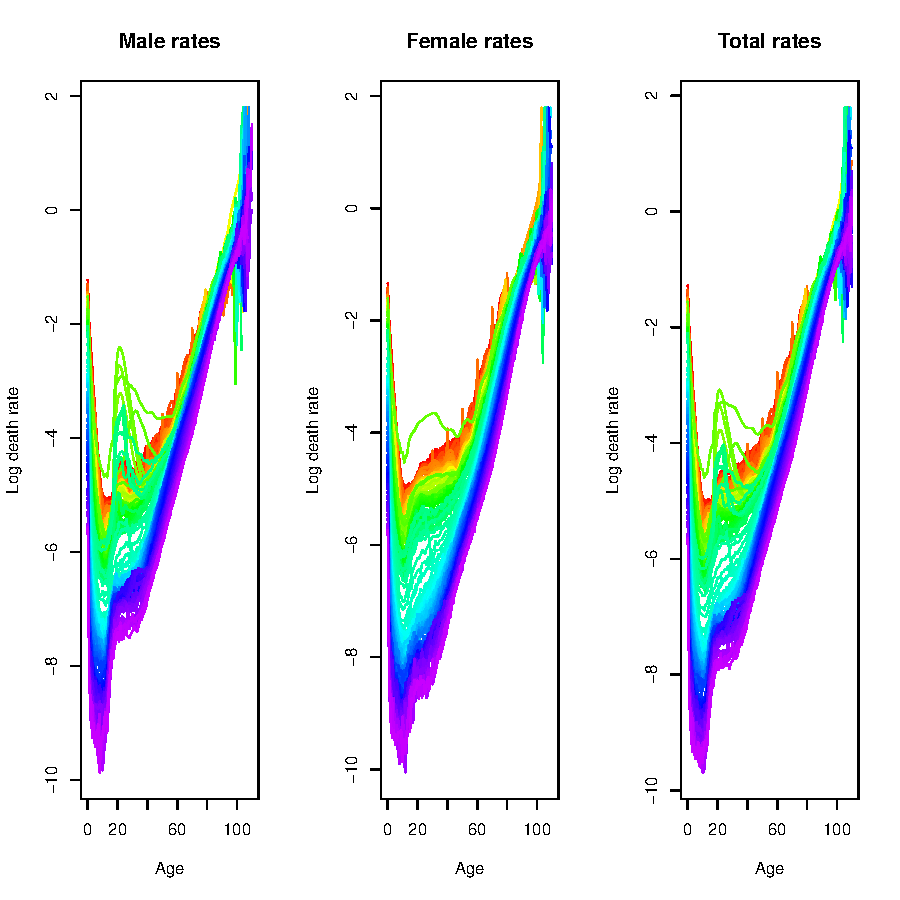
\includegraphics{mortality_projection-italyDemoFig}
\begin{Schunk}
\begin{Sinput}
R> par(mfrow=c(1,3))
R> plot(italyDemo,series="male",datatype="rate",
+      plot.type="time", main="Male rates",xlab="Years")
R> plot(italyDemo,series="female",datatype="rate",
+      plot.type="time", main="Female rates",xlab="Years")
R> plot(italyDemo,series="total",datatype="rate",
+      plot.type="time", main="Total rates",xlab="Years")
\end{Sinput}
\end{Schunk}
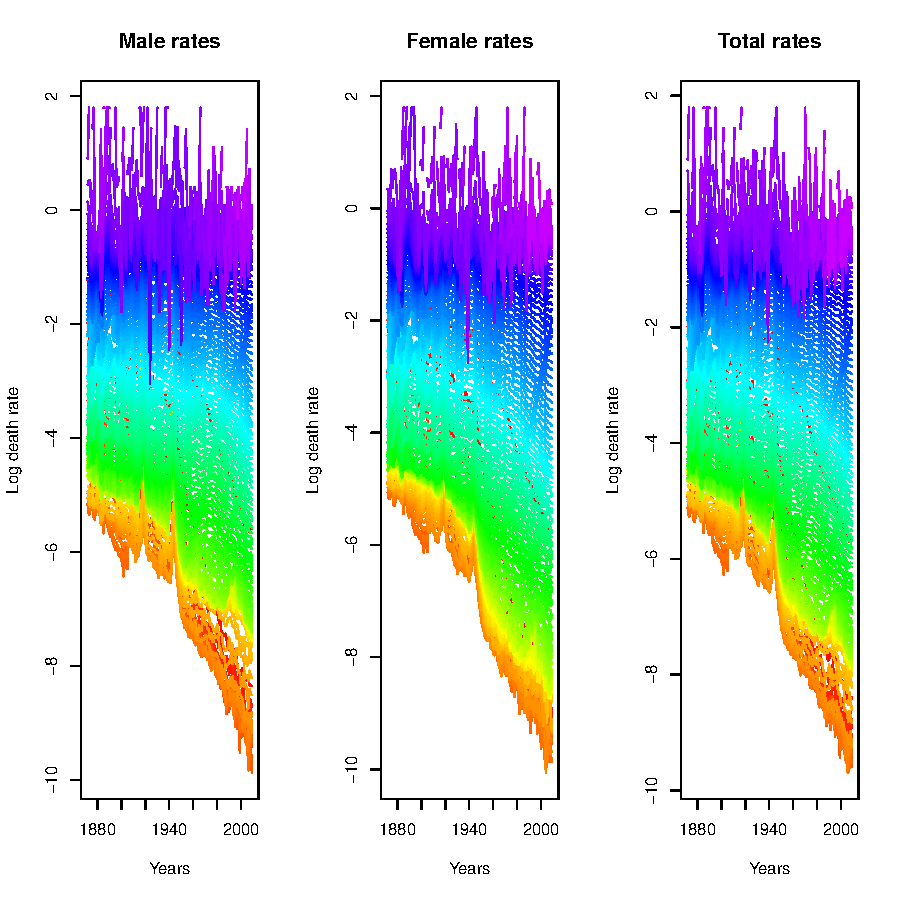
\includegraphics{mortality_projection-italyDemoFigTime}

Italian data confirms that mortality is falling at all ages with a different behaviour according to different ages

To fit Lee - Carter model (without going through logaritms) lca function can be used. Lee-Carter is here applied separately between male, female and total population and by considering a maximum age equal to 100.

\begin{Schunk}
\begin{Sinput}
R> italyLcaM<-lca(italyDemo,series="male",max.age=100)
R> italyLcaF<-lca(italyDemo,series="female",max.age=100)
R> italyLcaT<-lca(italyDemo,series="total",max.age=100)
\end{Sinput}
\end{Schunk}
%italyLcaT1<-lca(italyDemo,series="total",max#.age=100,adjust="dxt")
%italyLcaT2<-lca(italyDemo,series="total",max.age=100,adjust="none")

\textbf{lca} returned object allows us to inspect $a_x$, $b_x$ and $k_t$. Figures represent the values of the estimated parameters. 

\begin{Schunk}
\begin{Sinput}
R>   par(mfrow=c(1,3))
R>   plot(italyLcaT$ax, main="ax", xlab="Age",ylab="ax",type="l")
R>   lines(x=italyLcaF$age, y=italyLcaF$ax, main="ax", col="red")
R>   lines(x=italyLcaM$age, y=italyLcaM$ax, main="ax", col="blue")
R>   legend("topleft" , c("Male","Female","Total"),
+   cex=0.8,col=c("blue","red","black"),lty=1);
R>   plot(italyLcaT$bx, main="bx", xlab="Age",ylab="bx",type="l")
R>   lines(x=italyLcaF$age, y=italyLcaF$bx, main="bx", col="red")
R>   lines(x=italyLcaM$age, y=italyLcaM$bx, main="bx", col="blue")
R>   legend("topright" , c("Male","Female","Total"),
+   cex=0.8,col=c("blue","red","black"),lty=1);
R>   plot(italyLcaT$kt, main="kt", xlab="Year",ylab="kt",type="l")
R>   lines(x=italyLcaF$year, y=italyLcaF$kt, main="kt", col="red")
R>   lines(x=italyLcaM$year, y=italyLcaM$kt, main="kt", col="blue")
R>   legend("topright" , c("Male","Female","Total"),
+   cex=0.8,col=c("blue","red","black"),lty=1);
\end{Sinput}
\end{Schunk}
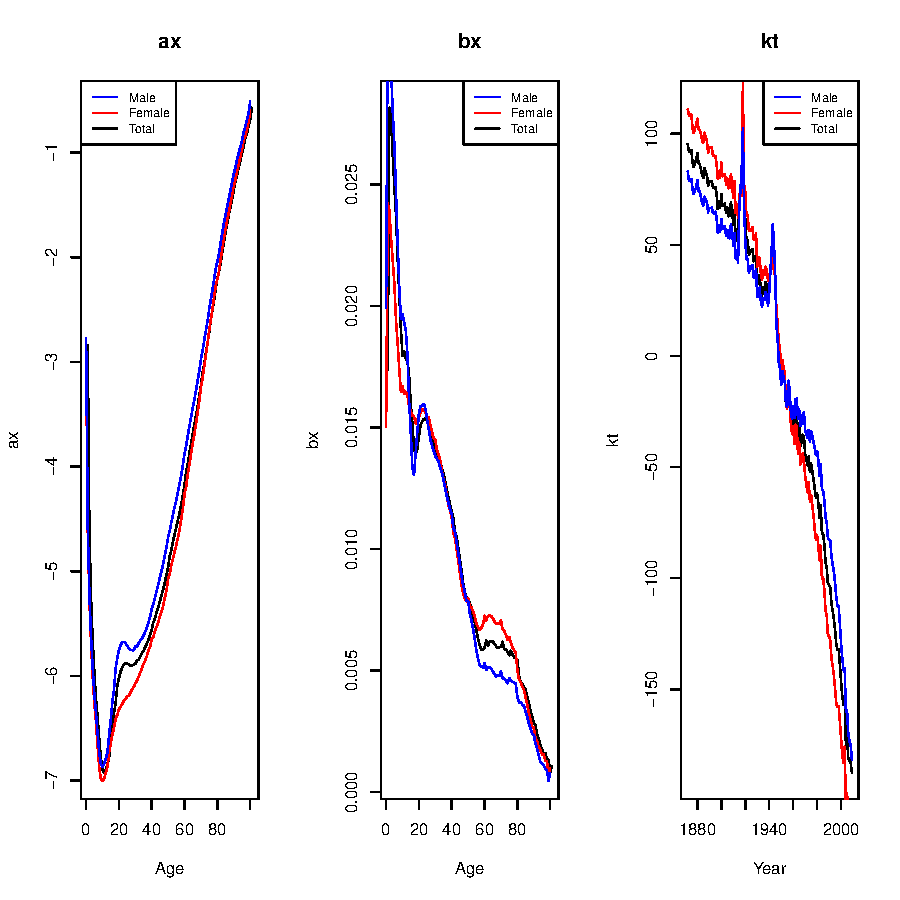
\includegraphics{mortality_projection-leeCarterResultsFig}

A similar behaviour of parameters is observed according to different data-sets. As expected the average mortality grows when age increases (see $\hat{a}_{x}$ pattern).Furthermore it is clearly visible the young mortality hump for males in the age-range (20,30) due to accidental deaths. $\hat{b}_{x}$ shows instead a greater value for younger ages and a greatest improvement for females in the age range (60-80).
Finally, as expected, $\hat{k}_{t}$ has a decreasing trend with the increment of time. \\

We can therefore use \pkg{forecast} package to project the future $k_{t}$s (up to 110). Projection is based on ARIMA extrapolation.
%ktTSeries<-italyLcaT$kt
%ktTArima<-auto.arima(ktTSeries,allowdrift=TRUE,max.order=20)
%ktTArimaForecasts<-forecast(ktTArima, h=110)
%fullKtT<-ts(c(ktTArimaForecasts$fitted, ktTArimaForecasts$mean),start=1872)  

\begin{Schunk}
\begin{Sinput}
R> fM<-forecast(italyLcaM,h=110)
R> fF<-forecast(italyLcaF,h=110)
R> fT<-forecast(italyLcaT,h=110)
\end{Sinput}
\end{Schunk}
%plot(forecast(italyLcaT,h=110))

The predicted values of $k_{t}$ rescaled to zero in the last observed year (2009) are here reported.

\begin{Schunk}
\begin{Sinput}
R> par(mfrow=c(1,3))
R> plot(fM$kt.f,main="Male")
R> plot(fF$kt.f,main="Female",)
R> plot(fT$kt.f,main="Total")
\end{Sinput}
\end{Schunk}
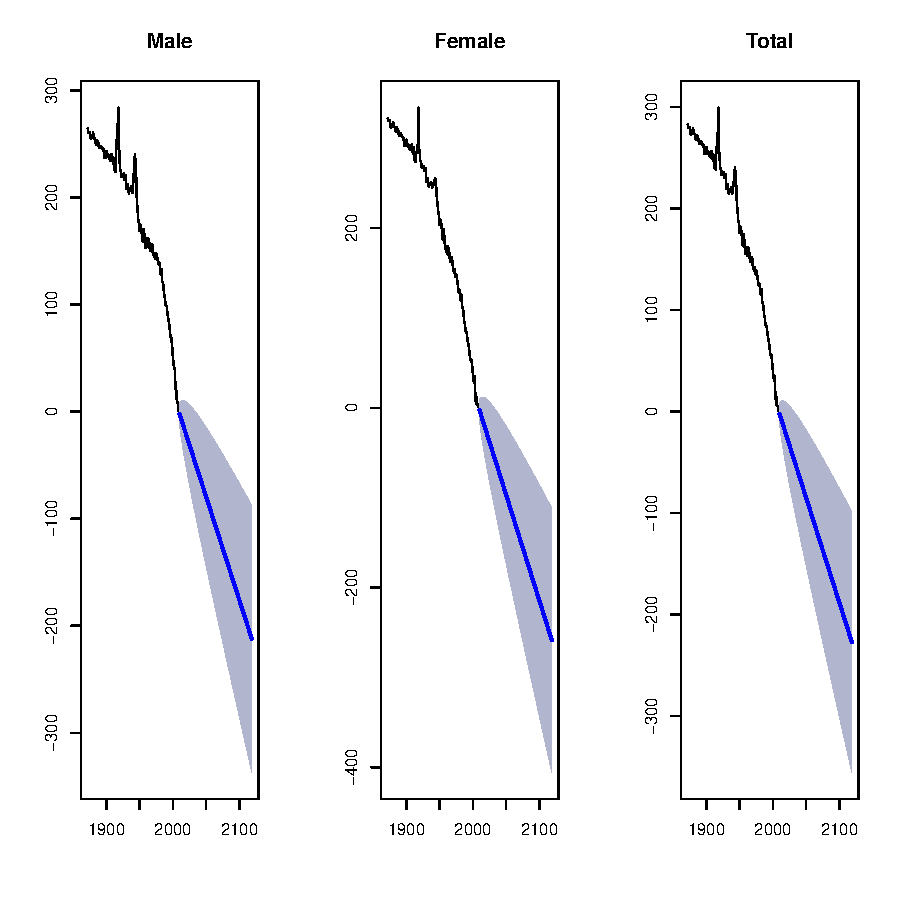
\includegraphics{mortality_projection-ktProjectionFig}

Finally, it's easy to derive the full pattern of rates. Past and forecasted rates are here binded in the same matrix.

\begin{Schunk}
\begin{Sinput}
R> ratesM<-cbind(italyDemo$rate$male[1:100,],fM$rate$male[1:100,])
R> ratesF<-cbind(italyDemo$rate$female[1:100,],fF$rate$female[1:100,])
R> ratesT<-cbind(italyDemo$rate$total[1:100,],fT$rate$total[1:100,])
\end{Sinput}
\end{Schunk}
%plot(italyDemo,series="total",main="Total: observed and forecasted rates",ylim=c(-20,2),lty=2)
%lines(fT,lty=2)
%max(unlist(fT$rate))
We report here the pattern of past and forecasted rates according to different population for people aged $65$. The expected improvement is clearly visible in the Figure.

\begin{Schunk}
\begin{Sinput}
R> par(mfrow=c(1,1))
R> plot(seq(min(italyDemo$year),max(italyDemo$year)+110),ratesF[65,],
+      col="red",xlab="Years",ylab="Death Rates",type="l")
R> lines(seq(min(italyDemo$year),max(italyDemo$year)+110),ratesM[65,],
+       col="blue",xlab="Years",ylab="Death Rates")
R> lines(seq(min(italyDemo$year),max(italyDemo$year)+110),ratesT[65,],
+       col="black",xlab="Years",ylab="Death Rates")
R> legend("topright" , c("Male","Female","Total"),
+        cex=0.8,col=c("blue","red","black"),lty=1);
\end{Sinput}
\end{Schunk}
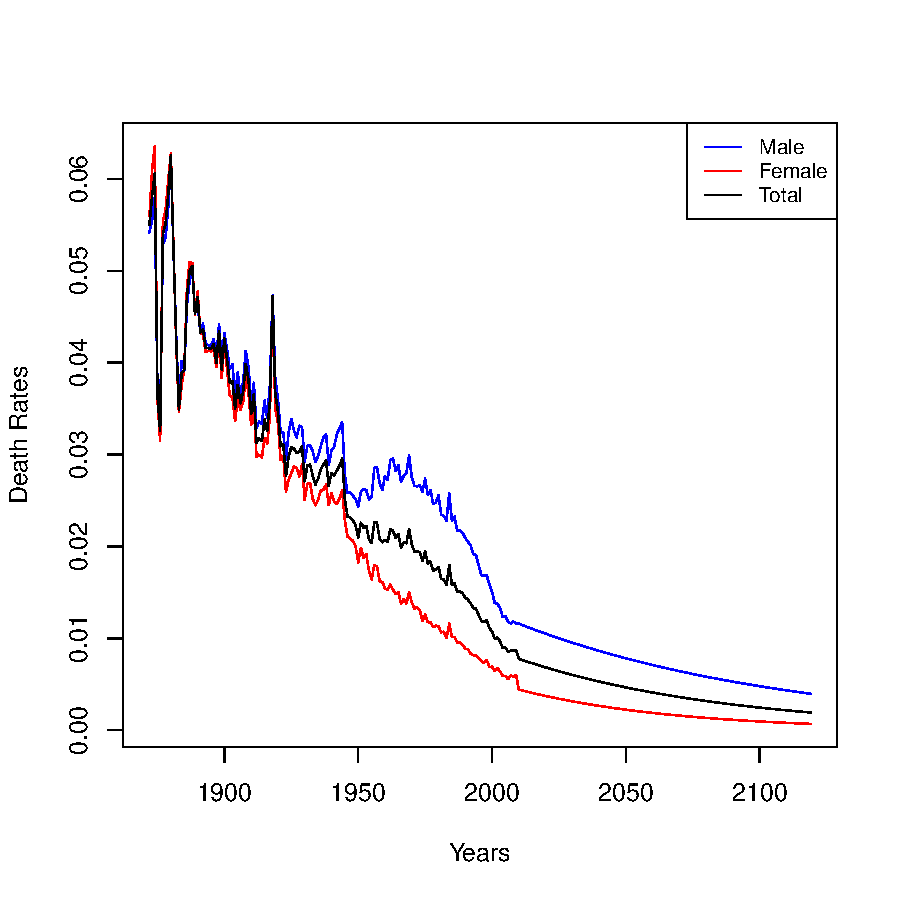
\includegraphics{mortality_projection-ktratesFig}

We have applied here the original version of Lee-Carter in order to obtain a forecast of mortality rates.
Alternative estimates can be derived by using \textbf{lca} function through the \pkg{demography} package (as Lee-Miller (\cite{LM}), Booth-Maindonald-Smith (\cite{BMS}) and Hyndman-Ullah (\cite{Hyn}) methods).
Finally Lifemetrics package allows to fit  \cite{BDV}, \cite{RH} and \cite{CBD} models.

\section{Perform actuarial projections}
Our aim is to create a function to project life table depending by year of birth,
using results from Lee - Carter model. 
In particular, for ages $0, 1, \ldots, \tau$ on which Lee-Carter model has been fit Equation~\ref{eq:fit1} apply, while for extreme
ages, $\tau + 1, \ldots, \omega$ on which no data were provided, it has been
assumed that on year probability decreases evenly in 20 steps.

\begin{equation}
\begin{array}{l}
\ln {\hat{\mu_{x,t}}} = \hat{a}_{x} + \hat{b}_{x}\hat{k}_{t}\\
\hat{p}_{x,t} = \exp \left(- \hat {\mu }_{x,t} \right)
\end{array}
\label{eq:fit1}
\end{equation}



\begin{Schunk}
\begin{Sinput}
R> createActuarialTable<-function(yearOfBirth,rate){
+ 
+   mxcoh <- rate[1:nrow(rate),(yearOfBirth-min(italyDemo$year)+1):ncol(rate)]
+   cohort.mx <- diag(mxcoh)
+   cohort.px=exp(-cohort.mx)
+   #get projected Px
+   fittedPx=cohort.px #add px to table
+ 	px4Completion=seq(from=cohort.px[length(fittedPx)], to=0, length=20)
+ 	totalPx=c(fittedPx,px4Completion[2:length(px4Completion)])
+ 	#create life table
+ 	irate=1.04/1.02-1
+ 
+ 	cohortLt=probs2lifetable(probs=totalPx, radix=100000,type="px", 
+   name=paste("Cohort",yearOfBirth))
+ 	cohortAct=new("actuarialtable",x=cohortLt@x, lx=cohortLt@lx, 
+ 	interest=irate, name=cohortLt@name)
+ 	return(cohortAct)
+ 	}
R> 
R> 
\end{Sinput}
\end{Schunk}

We can therefore calculate the APV of $\ddot{a}_{65}^{(12)}$ for the selected cohorts.
Values have been derived separately between males and females and by using directly the total population.

\begin{Schunk}
\begin{Sinput}
R> 	getAnnuityAPV<-function(yearOfBirth,rate) {
+ 		actuarialTable<-createActuarialTable(yearOfBirth,rate)
+ 		out=axn(actuarialTable,x=65,m=12)
+ 		return(out)
+ 	}
R> rate<-ratesM
R> for(i in seq(1920,2000,by=10)) {
+ 		cat("For cohort ",i, "of males the e0 is",
+ 		round(exn(createActuarialTable(i,rate)),2),
+ 		" and the APV is :",round(getAnnuityAPV(i,rate),2),"\n")
+ 		
+ 	}
\end{Sinput}
\begin{Soutput}
For cohort  1920 of males the e0 is 48.55  and the APV is : 3.92 
For cohort  1930 of males the e0 is 60.22  and the APV is : 5.03 
For cohort  1940 of males the e0 is 64.36  and the APV is : 5.63 
For cohort  1950 of males the e0 is 71.63  and the APV is : 5.92 
For cohort  1960 of males the e0 is 74.78  and the APV is : 6.22 
For cohort  1970 of males the e0 is 77.77  and the APV is : 6.52 
For cohort  1980 of males the e0 is 80.46  and the APV is : 6.81 
For cohort  1990 of males the e0 is 82.24  and the APV is : 7.1 
For cohort  2000 of males the e0 is 83.53  and the APV is : 7.38 
\end{Soutput}
\begin{Sinput}
R> rate<-ratesF
R> for(i in seq(1920,2000,by=10)) {
+   	cat("For cohort ",i, "of females the e0 at birth is",
+ 	round(exn(createActuarialTable(i,rate)),2),
+ 	" and the APV is :",round(getAnnuityAPV(i,rate),2),"\n")
+ 		
+ 	}
\end{Sinput}
\begin{Soutput}
For cohort  1920 of females the e0 at birth is 57.38  and the APV is : 6.21 
For cohort  1930 of females the e0 at birth is 66.99  and the APV is : 7.23 
For cohort  1940 of females the e0 at birth is 71  and the APV is : 7.8 
For cohort  1950 of females the e0 at birth is 78.22  and the APV is : 8.24 
For cohort  1960 of females the e0 at birth is 81.76  and the APV is : 8.63 
For cohort  1970 of females the e0 at birth is 84.54  and the APV is : 8.99 
For cohort  1980 of females the e0 at birth is 86.85  and the APV is : 9.33 
For cohort  1990 of females the e0 at birth is 88.18  and the APV is : 9.66 
For cohort  2000 of females the e0 at birth is 89.27  and the APV is : 9.96 
\end{Soutput}
\begin{Sinput}
R> rate<-ratesT
R> for(i in seq(1920,2000,by=10)) {
+     cat("For cohort ",i, "of total population the e0 is",
+ 		round(exn(createActuarialTable(i,rate)),2),
+ 		" and the APV is :",round(getAnnuityAPV(i,rate),2),"\n")
+ 		
+ 	}
\end{Sinput}
\begin{Soutput}
For cohort  1920 of total population the e0 is 52.85  and the APV is : 5.17 
For cohort  1930 of total population the e0 is 63.6  and the APV is : 6.23 
For cohort  1940 of total population the e0 is 67.73  and the APV is : 6.85 
For cohort  1950 of total population the e0 is 75.05  and the APV is : 7.24 
For cohort  1960 of total population the e0 is 78.42  and the APV is : 7.61 
For cohort  1970 of total population the e0 is 81.36  and the APV is : 7.96 
For cohort  1980 of total population the e0 is 83.93  and the APV is : 8.31 
For cohort  1990 of total population the e0 is 85.55  and the APV is : 8.64 
For cohort  2000 of total population the e0 is 86.81  and the APV is : 8.96 
\end{Soutput}
\end{Schunk}


\section*{Acknowledgments}\label{sec:acknowledgments}

The authors are deeply indebited with Prof. Rob J. Hyndman for his suggestions on these vignettes and to all people that contributed to \pkg{lifecontingencies} package.


\bibliography{lifecontingenciesBiblio}


\end{document}
